\begin{figure}[!t]
% \includesvg[width=1\textwidth]{figures/SAMIL_diagram_draft1.svg}
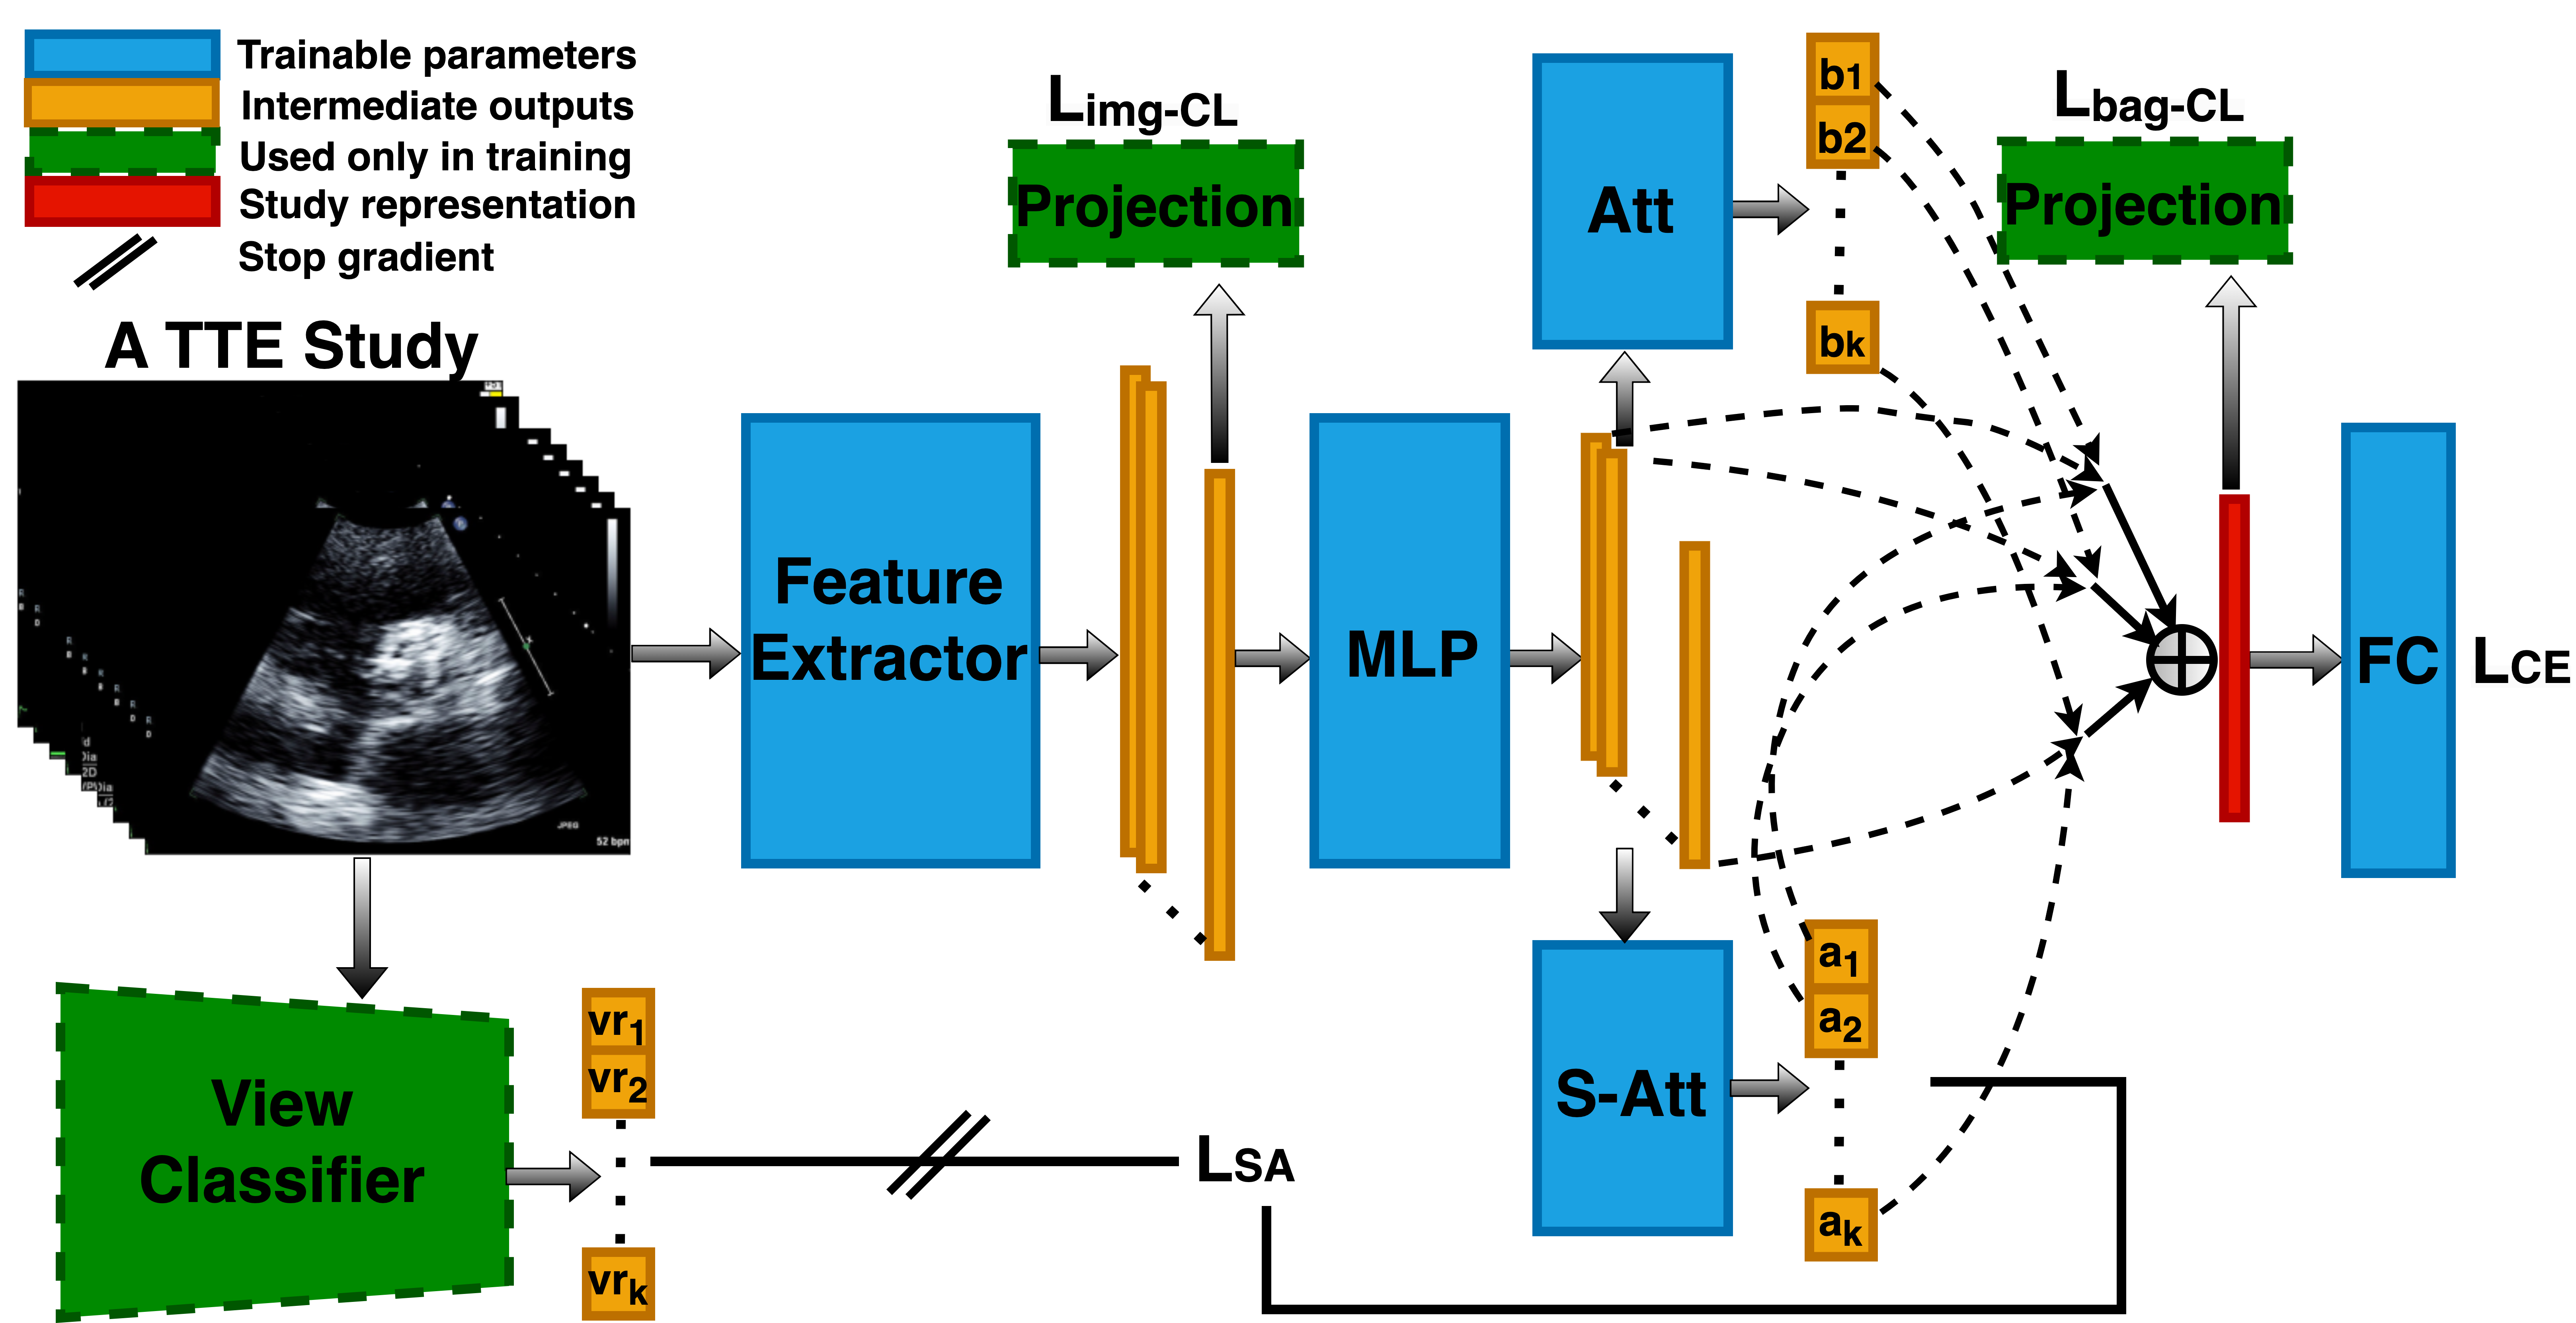
\includegraphics[width=1\textwidth]{figures/SAMIL_diagram_draft1.png}
\caption{\textbf{Overview of proposed method: Supervised Attention Multiple Instance Learning (SAMIL)}.
Given a study or ``bag'' with various images, a feature extractor processes each image individually into an embedding vector. Two attention modules (one supervised by a trained view classifier and one without) produce attention weights for each instance. The final study representation averages the image embeddings weighted by a combination of the two attentions (Eq.~\eqref{eq:patient_embedding_samil}). A fully connected layer then maps the study representation to a diagnosis label. 
\emph{Pretraining:} SAMIL can be pretrained using either bag-level (recommended, Sec.~\ref{sec:methods_CL}) or image-level contrastive learning. In either case, a projection head maps representations to a latent space where the contrastive loss is applied, following \citep{chen2020simple, chen2020improved}. The projection head is discarded after pretraining.
}%endcaption	
\label{fig:workflow_diagram}
\end{figure}